% For help on subfiles see https://www.sharelatex.com/learn/Multi-file_LaTeX_projects
\documentclass[../main.tex]{subfile}

\begin{document}
		
		\paragraph{} CuckooDroid is an extension of Cuckoo Sandbox the Open Source software for automating analysis of suspicious files. CuckooDroid brigs to cuckoo the capabilities of execution and analysis of android application \cite{cuckoodroid_docs}. For more information about the cuckoo sandbox, readers are encouraged to visit the cuckoo sandbox website \cite{cuckoo_website}. Currently, CuckooDroid only supports Android 4.1.
		
		\paragraph{} CuckooDroid can be downloaded from the CuckooDroid github repository \cite{cuckoodroid_github} by following the guidelines provided there. For more step-by-step installation guide, readers are encouraged to have a look at CuckooDroid documentation \cite{cuckoodroid_docs}. Because of changes in android emulator (goldfish) and android SDK the CuckooDroid documentation are not precisely accurate and some deviations are required from it in order to make the CuckooDroid work. By following the CuckooDroid documentation with a few changes discussed later in this chapter, it should be fairly easy for reader to configure his CuckooDroid setup. 

		
		\subsection{CuckooDroid architecture}
		\paragraph{} In this section we will describe the architecture of CuckooDroid. There are main two parts a "Host" and a "Guest". Below is an excerpt from the CuckooDroid documentation \cite{cuckoodroid_docs}:
		
		\say{This documentation refers to Host as the underlying operating systems on which you are running Cuckoo (generally being a GNU/Linux distribution) and to Guest as the Windows virtual machine used to run the isolated analysis.}
		
		\paragraph{} We will be configuring CuckooDroid with Android Emulator (Goldfish) and figure \ref{fig:cuckoodroid_avd_arch} shows the architecture CuckooDroid with Android Emulator. As it can be seen in the figure \ref{fig:cuckoodroid_avd_arch} that there are two main parts, Cuckoo Sandbox and Android Emulator.
		
		\begin{figure}
			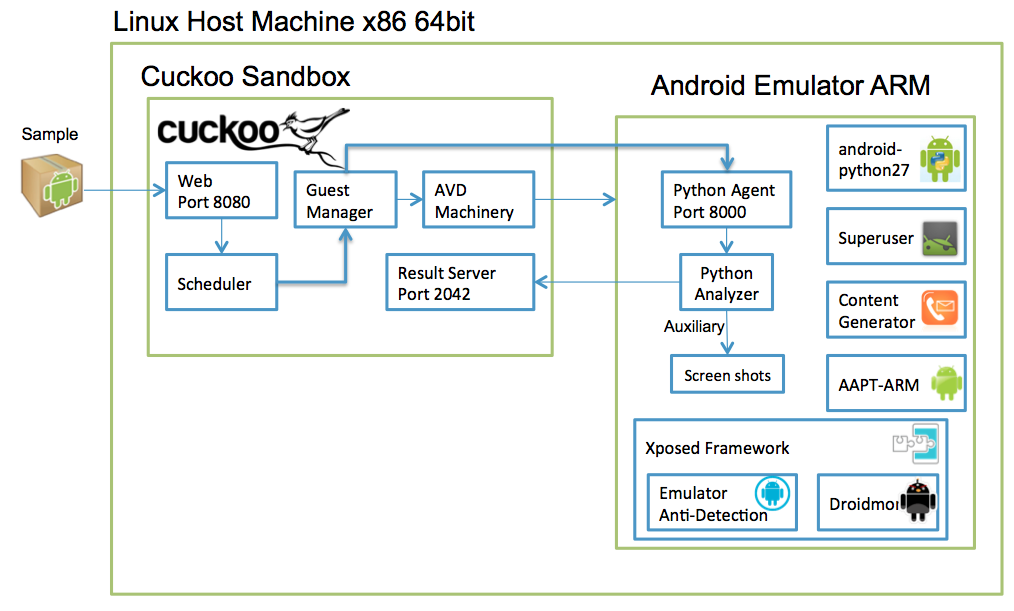
\includegraphics[width=\textwidth]{android_avd_arch.png}
			\caption{CuckooDroid architecture with AVD}
			\label{fig:cuckoodroid_avd_arch}
		\end{figure}
		
		\paragraph{} Cuckoo Sandbox is responsible for managing the android emulator and generating report at the end of analysis. Android Emulator executes the application, gather some information from it and reports it back to Cuckoo Sandbox. Below is the description of some of the main parts shown in figure \ref{fig:cuckoodroid_avd_arch}
		\begin{itemize}
			\item \textbf{Python Agent} Executed on AVD and is responsible for receiving APK file, Analysis code, configuration and executing analysis. It also provides constant status updates to Host.
			\item \textbf{Python Analyzer} Android analyzer component that is sent to the guest machine at the beginning of the analysis. This is the main part that executes application, send dropped files back to host, send screenshots back to host, interact with the application if required. It is also responsible for ending the analysis and sending back some log files back to host. It has modular structure and new modules can be added very easily.
			\item \textbf{Xposed Framework} A framework for modules that can change the behavior of the system and apps without affecting any APKs. The version in use only work up to Android 4.1.2 (API 16). In CuckooDroid two modules are used with this Framework:
			\begin{enumerate}

				\item \textbf{Droidmon:} Dalvik  API Call monitoring module, it hooks up API calls and prints it into logcat, anaylsis code takes it form logcat and store it in a log file which is sent back to host at the end of anaylsis.
				\item \textbf{Emulator Anti-Detection:} Implements some know Emulator Anti-detection techniques (For more details on this topic see Chapter \ref{sec:Chp4})
			\end{enumerate}
		\end{itemize}
		\paragraph{} In the rest of this chapter we will walk through configuring CuckooDroid and some of the changes which are necessary to make it work with latest Android Emulator and latest Android versions.
		\subsection{CuckooDroid Installation}\label{sec:cuckoodroid_installation}
		\paragraph{} Installation of CuckooDroid is pretty straight forward and can be easily done by following the Easy integration script available on the CuckooDroid github repository \cite{cuckoodroid_github}. For the configuration and requirements follow the instruction in the CuckooDroid documentations \cite{cuckoodroid_docs}. In the next two paragraphs we will give a bit more intuitive description of how CuckooDroid works which will help in understanding some of steps in installation and configuration step. Please note that there are some changes which are required to make CuckooDroid work and those are discussed in section \ref{sec:cuckoodroid_patching}.
		\paragraph{} The basic components of CuckooDroid can be seen in figure \ref{fig:cuckoodroid_avd_arch}. There are two basic parts of CuckooDroid host and guest. We run the cuckoo sandbox on host which handles the emulator. In order to do analysis our guest needs to be a rooted AVD with Xposed Framework \cite{xposed_module_repo} two of its modules Droidmon and Emulator Anti-Detection. We also need Python 2.7 to run the python agent and analyzer code on our guest.
		\paragraph{} Once we run the Cuckoo sandbox and submit a sample to it, it makes a new copy of our specified AVD and launches it. Once the machine boots, the cuckoo sandbox runs the python agent using Android Debugger (adb) and sends the APK file, configuration file, and analysis code to it and orders it to start executing the analysis code. The analysis code uses the apk module to install the sample and executes it. The DroidMon module of xposed Framework monitors the specified function calls using hooks and prints it on the logcat. Screenshot modules takes screenshots of the android screen and sends it to host. Once the analysis is completed, the analyzer sends all the required files back to host and terminates. Then host kills the emulator and starts making a report out of these files.
		\subsection{CuckooDroid required patching for Android 4.1}\label{sec:cuckoodroid_patching}
		\paragraph{} In this section we will talk about some of the changes which were required to make CuckooDroid work with Android 4.1. There are two main steps, one is the persistent root problem and the second one is some bug fixes in python analyzer code.
		
		\subsubsection{Android 4.1 Persistent Rooting}
		\paragraph{} Now coming towards the first fix which was that the root wasn't staying persistent across reboots. It was the result of changes in Android emulator. More details and solutions about this problem can be found in issue 4 of CuckooDroid github repository \cite{cuckoodroid_root_issue}. The solution can be found in the same issue, according to which we needed to copy the system.img file from the android SDK directory to the AVD directory. The following command can be used to do that, make sure you replace the paths according to the location of your android SDK and AVD.
		
		\begin{lstlisting}
			$ cp ~/Android/Sdk/system-images/android-16/default/armeabi-v7a/system.img ~/.android/avd/aosx.avd/system-qemu.img
		\end{lstlisting}
		
		\paragraph{} After the above step, we need to start the emulator with command given below:
		\begin{lstlisting}
			$ emulator -avd aosx -qemu -nand -system,size=0x1f400000,file=~/.android/avd/aosx.avd/system-qemu.img&
		\end{lstlisting}
		
		The follow the standard steps of rooting described in cuckoodroid documentations \cite{cuckoodroid_docs}. I also made some youtube tutorials to help the readers with the process. You can find the related video tutorial here \cite{rooting_youtube}
		
				
		\subsubsection{Bug fixes in Analyzer code}
		\paragraph{} The second fix is in the python code that is executed on Android. The CuckooDroid analyzer and agent code heavily relies on Subprocess Management library \cite{subprocess_management_library} (specifically subprocess.Popen() method). During debugging we noticed that Most of the calls to subprocess.Popen() method never returns resulting in analysis critical time out. Upon further research we found an issue relating to a similar problem in python 3.7 \cite{subprocess.popen_issue16255}, which seems to be the case here. The subprocess.Popen function uses /bin/sh in Unix environments. Android is detected as a Unix environment, but has moved that executable to "/system/bin/sh". This can be worked around by adding a parameter executable="/system/bin/sh" to all the subprocess.Popen calls. One related problem was that in some parts of the analyzer, like in adb.py os.popen was used to execute shell commands. This function was also failing to return so we have to replace it with subprocess.Popen. The video related video tutorial can be found here \cite{subprocess_youtube}
		
		\paragraph{} The next limitation that we faced was that CuckooDroid only supports Android upto 4.1, which is quiet older and in order to analyze applications that are targeting higher version of androids we need to find a way to run CuckooDroid on higher version of Androids. In the next sections we will describe the steps and results of our attempts to upgrade to Android 5.1 and Android 7.0.

		\subsection{CuckooDroid with Android 5.1}
		\paragraph{} Just like with Android 4.1, here we again faced the persistent root problem. Another problem was that we couldn't use the python binaries for android that comes with CuckooDroid because from this version Android make it a requirement for binaries to support PIE mode. In the following subsections we will describe in more detail about how did we solved these problems. Here we used the x86 image just to save time during testing. This rooting procedure works on arm image too but that speed of arm image is very slow and was wasting a lot of time during the development and debugging.
		
		\subsubsection{Android 5.1 AVD persistent rooting procedure} \label{sec:android_5.1_root}
		\paragraph{} The rooting procedure for Android 5.1 is a bit different than that of Android 4.1 in the sense that we needed updated version of tools like SuperSU, XposedFramework etc. Below are the required steps to root Android 5.1 AVD and keep the root persistent.
		\begin{enumerate}
			\item First copy the system.img to your avd directory and rename it as system-qemu.img: For example for Nexus One API 22 x86: \newline 
			\begin{lstlisting}[language=bash]
			cp ~/Android/Sdk/system-images/android-22/default/x86/system.img ~/.android/avd/Nexus_One_API_22_x86.avd/system-qemu.img
			\end{lstlisting}
						
			
			\item Then start the AVD Machine with \newline 
			\begin{lstlisting}[language=bash]
			emulator @Nexus_One_API_22_x86 -verbose -writable-system
			\end{lstlisting}
						
			
			\item Run the script located in utils/android\textunderscore emulator\textunderscore creator and named create\textunderscore guest\textunderscore avd\textunderscore x86/arm\textunderscore 5.1+.sh. Below is a snippet from one of the scripts which was made with the help of stackexchange answer by a user with the name xavier\textunderscore fakerat \cite{android_emulator_7.1_root_stackexchange} \newline
			\begin{lstlisting}[language=bash]
			#!/usr/bin/env bash
			# Inspired by: https://android.stackexchange.com/questions/171442/root-android-virtual-device-with-android-7-1-1/176447
			#this script is meant for easy creation on an analysis machine for android emulator avd
			
			#Path to the local installation of the adb - android debug bridge utility.
			#ADB=/home/wra/Andriod/Sdk/platform-tools/adb
			ADB=$(which adb)
			if [ ! -f $ADB ]
			then
			echo -e "\n-Error: adb path is not valid."
			exit
			fi
			echo -e "\n-adb has been found."
			# First we root the emulator using Superuser
			echo -e "\n-Pushing /system/xbin/su binary"
			$ADB root
			$ADB remount
			# one of these is correct, we do both just to be on safe side
			$ADB push nougat/SuperSU-v2.82-201705271822/x86/su.pie /system/xbin/su
			$ADB shell chmod 06755 /system/xbin/su
			$ADB push nougat/SuperSU-v2.82-201705271822/x86/su.pie /system/bin/su
			$ADB shell chmod 06755 /system/bin/su
			echo -e "\n-Installing application Superuser"
			$ADB install nougat/eu.chainfire.supersu_2.82.apk
			# Install Xposed Application
			echo -e "\n-Installing Xposed Application"
			$ADB install nougat/XposedInstaller_3.1.4.apk
			# Install Droidmon Application
			echo -e "\n-Installing Droidmon Application"
			$ADB install hooking/Droidmon.apk
			# Install Termux application
			$ADB install nougat/com.termux.apk
			# Install Anti Emulator Detection Application
			echo -e "\n-Installing Anti Emulator Detection Application"
			$ADB install hooking/EmulatorAntiDetect.apk
			$ADB push anti-vm/fake-build.prop /data/local/tmp/
			$ADB push anti-vm/fake-cpuinfo /data/local/tmp/
			$ADB push anti-vm/fake-drivers /data/local/tmp/
			# Install Content Generator
			echo -e "\n-Installing Content Generator"
			$ADB install apps/ImportContacts.apk
			# Install Cuckoo Agent and Python for ARM
			echo -e "\n-Pushing Agent executing scripts"
			$ADB push ../../agent/android/python_agent/. /data/local/ 
			$ADB shell chmod 06755 /data/local/aapt
			$ADB shell chmod 06755 /data/local/get_terminal.sh
			$ADB shell chmod 06755 /data/local/run_agent.sh
			echo -e "\n***** Run the following commands and you are good to go*****\n"
			echo "adb shell"
			echo "cd /system/bin/"
			echo "su root"
			echo "su --install"
			echo "su --daemon&"
			echo "setenforce 0"
			echo -e "\n"
			echo -e "*NOTE"
			echo " To make sure everything is working fine after the rooting is done, do the following:"
			echo " Open android emualtor and run termux. Then type python2 to make sure to that python is installed"
			echo " Then open adb shell Run the get_terminal.sh script and then type python2 to verify that you "
			echo " that you can run python with root previledges. After that run run_agent.sh and verify that agent is running."
			\end{lstlisting}
			
		\item Run the SuperSu app and if the device is rooted, it will ask for update, update the app, don't reboot yet.
		\item After update, open Xposedframework app and click install there, it will ask for administrator permission, click grant.
		\item Enable Droidmon and anti-emulator modules.
		\item Soft reboot the machine, (It will be somewhere in xposed app)
		\item After reboot verify root by opening SuperSU app and it doesn't give you an error and show xposedframework app, the device is rooted.
		\item Close the machine, (The emulator 27.0.1 will save the snapshot of the machine and will load it at next start)
		\item start the machine with -writable-system option (without it the loaded machine is not rooted)and it will automatically load the previously save snapshot, that means it will be up and running in no time. (verify root by opening SuperSu app), then close the machine.
		\item start the machine again with adding one more option to above command, that is -no-snapshot, this time the machine is boot properly and verify the root by running SuperSU app.
					
		\end{enumerate}
		\subsubsection{Python 2.7 on Android 5.1} \label{sec:android_5.1_python}
		\paragraph{} In order to do the analysis we need to have python 2.7 in our Android 5.1 guest. CuckooDroid comes with python 2.7 binaries which are compiled for Android 4.1, which doesn't work with Android 5.1 because with the release of Android 5.1 Android requires all dynamically linked executables to support PIE (position-independent executables). So we either need python compiled with PIE support. We can either compile it ourselves or we can use pre-compiled python with PIE support. We opted for the pre-compiled solution because of simplicity. Below is an example on how to compile a C program with PIE support using Android Native Development Kit (NDK).
		
		\paragraph{Compiling C code for Android 5.1+}
		\begin{enumerate}
				\item Download and extract NDK (My NDK directory is ~/android-ndk-r16)
				\item Create a new standalone toolchain using the script ~/android-ndk-r16/build/tools/make\textunderscore standalone\textunderscore toolchain.py
				\begin{lstlisting}[language=bash]
				python ~/android-ndk-r16/build/tools/make_standalone_toolchain.py --arch x86 --api 22 --install-dir ~/android-ndk-r16/toolchains/x86-22
				\end{lstlisting}
				\item Write your c program, compile it and link it separately with required flags for PIE.
				\begin{lstlisting}[language=bash]
				cd ~/android-ndk-r16/toolchains/x86-22/bin
				touch main.c
				cat > main.c
				
				#include<stdio.h>
				int main()
				{
				printf("Hello world!\n");
				return 0;
				}
				
				./i686-linux-android-gcc -c main.c  -fPIE
				./i686-linux-android-gcc -lm main.o -pie
				\end{lstlisting}
				\item Start emulator, copy file to it, make it executable and run it
				\begin{lstlisting}[language=bash]
				emulator @Nexus_One_API_22_x86 -writable-system
				adb push a.out /data/local
				adb shell chmod 06755 /data/local/a.o
				adb shell /data/local/a.o
				WARNING: linker: /data/local/a.out: unused DT entry: type 0x6ffffffe arg 0x32c
				WARNING: linker: /data/local/a.out: unused DT entry: type 0x6fffffff arg 0x1
				Hello world!
				\end{lstlisting}
		\end{enumerate}
		
		\paragraph{Pre-Compiled python for Android 5.1+}
		\paragraph{} Now, as we said above we used the pre-compiled python 2.7 that can be installed inside the Termux application \cite{termux_website}. Termux is an Android terminal emulator and Linux environment application that provides several linux command line tools an android making it really powerful. The app doesn't require root permissions which means it can't access or modify files outside of application. We needed a workaround so that we can run termux shell as root and have access to all system. Below are steps required to achieve that:	
				
		\begin{enumerate}
		\item Download Termux apk from google playstore or apkmirror and install it to rooted emulator
		\item Open the installed app and type "pkg search python"
		\item Install python2 using pkg install python2 (take help from step2 to determine exact command)
		\item Now type python2 and you will have a working python. But this only works inside the app and can't be run as sudo/root.
		\item To be able to run python as root from adb, we will need to download the script https://github.com/cswl/tsu (A fork of this which support optional command is here https://github.com/kiney/tsu)
		\item Push this script to your emulator and run it with -e option.
		\item It will give you a bash shell (whatever) which support most of linux commands and others can be installed as well. (You need to have rooted device to run this script)
		\item Now we need to add the code inside the script so that instead of launching a shell it run our agent.py script.
		\item To do that go to line 100 which is:
		\begin{lstlisting}[language=bash]
		exec "$s" --preserve-environment -c "LD_LIBRARY_PATH=$LD_LIBRARY_PATH $ROOT_SHELL" 
		\end{lstlisting}
		Step 10: Edit the line as follows:
		\begin{lstlisting}[language=bash]
		exec "$s" --preserve-environment -c "LD_LIBRARY_PATH=$LD_LIBRARY_PATH python2 /data/local/agent.py" 
		\end{lstlisting}
		
		\item Now run this script with "-e" and you will see that our agent.py script is been fired.
		\item Now we need to change part of the code which fires up agent.sh
		\item Due to some unknown reasons we ran into some permissions problems like not being able to read hooks.json file. In logcat droidmon was complaining about not having permission to read hooks.json. This can be fixed by setting the global read flag on hooks.json after it is copied in cuckoodroid/analyzer/android/analyzer.py Below is the snippet of code:
		\begin{lstlisting}[language=python]
		def prepare(self):
			# Initialize logging.
			init_logging()
			
			# Parse the analysis configuration file generated by the agent.
			self.config = Config(cfg="analysis.conf")
			
			# We update the target according to its category. If it's a file, then
			# we store the path.
			if self.config.category == "file":
			self.target = os.path.join("/data/local/tmp", str(self.config.file_name))
			shutil.copyfile("config/hooks.json", "/data/local/tmp/hooks.json")
			os.chmod("/data/local/tmp/hooks.json", 0754) # Give set global read flag on hooks.json
			# If it's a URL, well.. we store the URL.
			else:
			self.target = self.config.target
		\end{lstlisting}
		
		\item Another problem was in the screenshot module, it wasn't able to read to screenshots taken and this can be solved by using the same method as above i.e, setting global read at the time the file is created and also changing the location of file in this case sdcard was readonly and this function wasn't able to save the image there. Below is the modified code of take\textunderscore screenshot() method in adb file:
		\begin{lstlisting}[language=python]
			def take_screenshot(filename):
				proc1= subprocess.Popen("/system/bin/screencap -p /data/local/screenshots/"+filename, # "/data/local/screenshots/" Fix for /sdcard read only
				stdout=subprocess.PIPE,
				shell=True,
				stderr=subprocess.PIPE,
				executable='/system/bin/sh')
				stdout, stderr = proc1.communicate()
				
				if len(stdout)>0:
				log.info("take_screenshot stdout: %s", stdout)
				if len(stderr)>0:
				log.info("take_screenshot stderr: %s", stderr)
				
				os.chmod("/data/local/screenshots/"+filename, 0744)
				return "/data/local/screenshots/"+filename
		\end{lstlisting}
		
		\end{enumerate}
		
		\subsection{CuckooDroid with Android 7.0}
		\paragraph{} We didn't have much success with Android 7.0. We could't pass the persistent rooting problem and the machine wouldn't boot after the rooting procedure as described for Android 5.1.
		
		\subsection{Chapter Conclusion}
		\paragraph{} After the work described in this chapter we came to some conclusions which will be described in this section.
		\paragraph{Emulator Anti Detection} Although during our dynamic analysis we didn't analyzed enough malicious samples make an estimate of the usage of emulation detection techniques in these samples, but a little search on the Internet revealed a several techniques that were very easy to implement and or integrate into an application and we reached the conclusion that it can be very easy for a determined threat actor to evade analysis and thus can make its way to popular android application distribution paltforms like google play store. We will give a bit more information about this topic in the next chapter.
		
		%\todo[inline]{Frida good because can adapt quickly to new threats and good support for higher version of android}
		\paragraph{Support for higher version android} We also reached a conclusion that there is dire need for android malware analysis paltforms that run latest android operating systems. We identified Frida, a dynamic instrumentation framework as a best candidate for instrumentation in CuckooDroid, because it is well maintained and support latest android operating systems.
		
		\paragraph{Slow emulator performance} With the android emulators running higher versions of Android, there is big performance penalty. Running an arm image of android on x86 based PC system is also one of the reason of performance degradation. One solution to the problem can be using Houdini translation that allows android apps written for arm processors to be executed on x86 android image. We didn't investigated this solutions further and can be done as a separate project. \todo[inline]{Add to future work}

\end{document}